  \section[3M\textsuperscript{\texttrademark} Healthcare Data Dictionary (HDD)]
  {3M HDD\textsuperscript{\texttrademark}}
  \label{sec:hdd}
  
  \initial{H}\textit{ealthcare Data Dictionary (HDD )}\
  is a controlled medical vocabulary server; makes it possible to map and manage\
  medical terminologies, integrate content and standardize healthcare data. Allows\
  organizations to transmit and receive accurate, actionable patient data across\
  systems and applications, regardless of where data\
  originates~\citep{_3M_Healthcare_Data_Dictionary_2013}.\\
  
  \noindent HDD incorporates and links terms from multiple clinical information\
  systems and standard terminologies. It maps disparate medical terms to\
  give data context and meaning; and is used to standardize data to make\
  it more interoperable and computable. It is a concept-based vocabulary and\
  knowledge base. \citep{_3M_Healthcare_Data_Dictionary_2013}.\\

  \noindent In June 2012, the U.S. Department of Defense and the Department\
  of Veterans Affairs reached an agreement with Salt Lake City-based 3M Health\
  Information Systems to make HDD freely available as open-source content and\
  software. HDD, which has been deployed since 1996 by 3M under an agreement with\
  the DoD and VA, was started as a development project to standardize clinical information.\
  All major healthcare standard technologies are mapped unto HDD:\
  SNOMED CT\textsuperscript{\ref{sec:snomedct}}, LOINC\textsuperscript{\ref{sec:loinc}},\
  ICD-9 and ICD-10\textsuperscript{\ref{sec:icd}}.\citep{_DeGaspari_2013}\
 
  \subsection{Information Models, Knowledge Base, Vocabulary}\

  \begin{figure}[ht!]
    \label{fig:ikv}
    \centering
    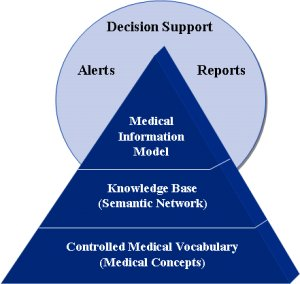
\includegraphics[scale=0.75]{hdd.jpg}
    \caption{Key Components of HDD}\citep{_3M_HDD_Product_Overview_2010}\
  \end{figure}  

  \begin{itemize}
    \itemsep0ex
    \item  \textbf{Information Models:} describes relationships among events and terminologies in a way that\
    gives them meaning and context. IM's mediate between data gathering software and databases\
    and are supported by terminologies.\\

    \item  \textbf{Knowledge Base:} defines the domains referenced by the information models.\
    Domains are created and populated by the web of relationships among concepts.\
    Semantic relationships fall into two broad categories: hierarchical and non hierarchical.\\

    \noindent HDD's knowledge base consists of semantic networks and hierarchies that describe\
    the complex relationships existing between concepts in the vocabulary. These\
    relationships can be hierarchical (``parent-child'' or ``is-a'') or\ 
    non-hierarchical ``is-a-component-of''. Figure 6 (below) is an example of how\
    the knowledge base can describe the\ relationships between the components of a\
    CHEM 4 laboratory test.\citep{_3M_HDD_Product_Overview_2010}\
    
     \begin{figure}[ht!]
      \label{fig:lab}
      \centering
      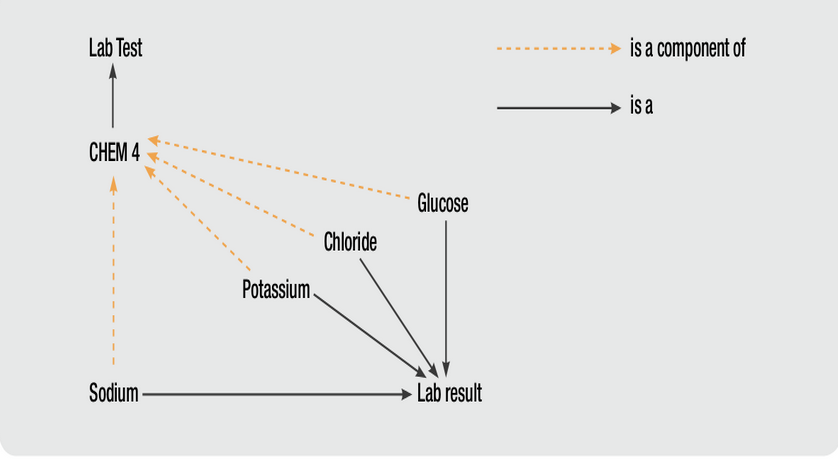
\includegraphics[scale=0.4]{labtest.png}
      \caption{Sample of HDD's knowledge base as applied to CHEM 4 lab test}\
      \citep{_3M_HDD_Product_Overview_2010}\
    \end{figure}  


    \item \textbf{Vocabulary:} Identifies medical concepts and organizes them\
    to support synonyms, multiple surface forms, and other lexical\
    characteristics. The HDD is a controlled medical vocabulary that follows\
    best medical informatics practices such as concept permanence, multiple\
    hierarchies, and meaningless identifiers. Each unique concept in the HDD\
    is assigned a Numeric Concept Identifier (NCID) code.\citep{_3M_HDD_Product_Overview_2010}\
  \end{itemize}

  \subsection{How we can use it}
  The server is the complete repository of concepts and associations, maintained and made available for download\
  in its most up-to-date version. Organizations can download and install the package locally to ensure constant\ 
  access to its contents. Users of the HDD will have the ability to request additions to the dictionary, which the team\
  at 3M will review and determine if they should be included.\citep{_Murphy_2012}\
  
 \subsection{Architecture and Platform Independence}
  HDD was designed to meet open architecture standards, allow for platform\
  independence, and conforms to the following industry standards:\
  \begin{itemize}
    \itemsep0ex
    \item Linux platform\
    \item HL7 Common Technology Services (CTS)\
    \item HL7 messaging\
    \item Abstract Syntax Notation (ASN.1) information model. transferable to XML\
    \citep{_3M_HDD_Product_Overview_2010}\
  \end{itemize}

  \begin{figure}[ht!]
    \label{fig:asn}
    \centering
    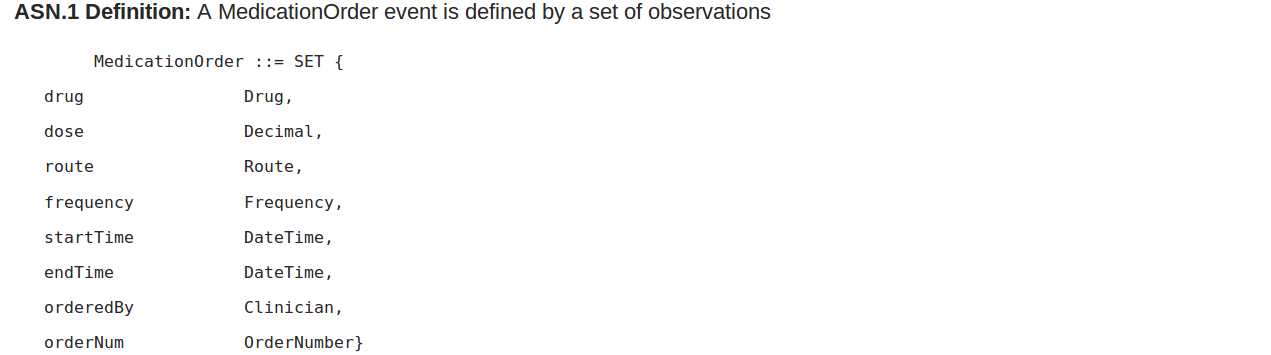
\includegraphics[scale=0.4,trim=1 1 400 1,clip]{asn.png}
    \caption{Simplified ASN.1 definition}\
    \citep{_3M_HDD_Product_Overview_2010}\
  \end{figure}  

  \begin{figure}[ht!]
    \label{fig:sid}
    \centering
    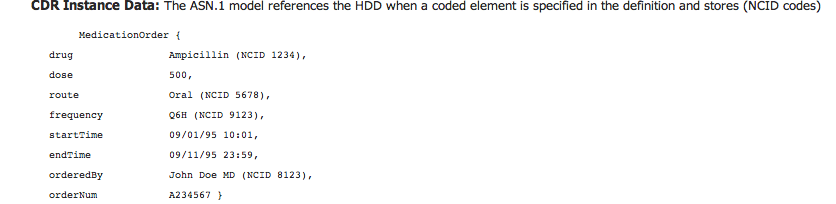
\includegraphics[width=\textwidth]{sid.png}
    \caption{Sample instance data}\
    \citep{_3M_HDD_Product_Overview_2010}\
  \end{figure}  
 
  \subsection{Mapping Source Controlled Medical Vocabularies (CMV's) and Local Vocabularies}
  All industry-standard CMVs can coexist in the 3M HDD because of a process\
  called mapping, which cross-references elements in each CMV with a concrete,\
  unambiguous concept in the 3M HDD.\\
  \citep{_3M_HDD_Product_Overview_2010}\

  \begin{figure}[ht!]
    \label{fig:cid}
    \centering
    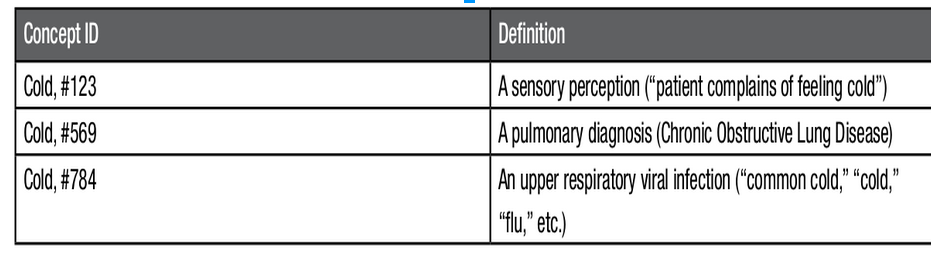
\includegraphics[scale=0.4]{conceptid.png}
    \caption{Sample of HDD's concepts and NCIDs}\
    \citep{_3M_HDD_Product_Overview_2010}\
  \end{figure}  
